\chapter{Evaluación}
\label{cap:evaluacion}
Una vez terminado el desarrollo de AdaptaMaterialEscolar 2.0, llevamos a cabo una evaluación para evaluar si nuestro proyecto resultaba útil para los docentes que necesitaban realizar adaptaciones curriculares para sus estudiantes en cualquier etapa académica. Con el propósito de realizar una valoración detallada, nos enfocamos en evaluar varios aspectos de nuestro proyecto: el diseño de la interfaz, la usabilidad del sistema en su totalidad y de cada funcionalidad de manera independiente y detectar posibles mejoras que podrían implementarse en el futuro.

A continuación se explica el diseño de la evaluación (Sección \ref{sec:disenyoEvaluacion}), los resultados obtenidos  (Sección \ref{sec:resultadosEvaluacion}) y las conclusiones obtenidas (Sección \ref{sec:conclusionesEvaluacion}).

\section{Diseño}\label{sec:disenyoEvaluacion}
Con el fin de permitir a los usuarios finales evaluar nuestra aplicación, creamos un examen de prueba y una hoja de apuntes sobre las asignaturas de conocimiento del medio y matemáticas.
Para facilitar la evaluación y el análisis de los resultados de nuestra aplicación web, creamos una encuesta\footnote{\url{https://docs.google.com/forms/d/e/1FAIpQLSdg7mGUfGBW5LoGIWulEUq-vhloL5rlkU_aIZCUzpqiJp164A/viewform?usp=sf_link}} en Google Forms dirigida a los usuarios finales. Durante la evaluación, los usuarios experimentaban directamente con las diversas funcionalidades, tratando de replicar el examen y la hoja de apuntes proporcionados.

La evaluación se ha diseñado de la siguiente manera:
\begin{itemize}
    \item La evaluación comienza con varios párrafos agradeciendo la colaboración de los usuarios, explicando la herramienta que están a punto de probar y proporcionando un resumen de la estructura de la evaluación. Además, se solicitó a los usuarios que dieran su consentimiento para el tratamiento de los resultados obtenidos en la evaluación.
    \item A continuación, se realizarán unas preguntas de screening y demográficas para el posterior análisis de los datos.
          \begin{itemize}
              \item ¿Cuántos años tienes?
              \item ¿Eres docente?
              \item ¿Eres estudiante de magisterio?
              \item ¿Podrías decirnos en qué nivel del sistema educativo eres docente?
              \item ¿Has tenido que hacer alguna adaptación curricular no significativa?
              \item ¿Cuántas veces?
          \end{itemize}
    \item Después, el evaluador debía crear un examen con preguntas de todos los tipos posibles. En este apartado se les proporcionó a los usuarios un examen creado con AdaptaMaterialEscolar 2.0 para que tratasen de replicarlo (en el Apéndice \ref{ape:examenEvaluacion} se muestra el examen que se proporcionó a los evaluadores). Tras terminar de crear cada ejercicio, los usuarios debían responder el test de usabilidad ASQ\footnote{\url{https://help.qualaroo.com/hc/en-us/articles/360039070552-After-ScenarioQuestionnaire-ASQ}} (After Scenario Questionnaire), el cual permite al usuario evaluar la dificultad de cada una de ellas. Este cuestionario ha de ser respondido una vez finalizada cada tarea y está compuesto por tres afirmaciones. El usuario ha de indicar cuán de acuerdo está mediante una escala Likert de 1 a 5, siendo el 1 muy en desacuerdo y el 5 muy de acuerdo. Dichas afirmaciones son:
          \begin{itemize}
              \item En general, estoy  satisfecho o satisfecha con la facilidad de completar esta tarea.
              \item En general estoy  satisfecho o satisfecha con la cantidad de tiempo que me ha llevado completar esta tarea.
              \item Estoy  satisfecho o satisfecha con la respuesta de la aplicación al realizar las acciones, sé lo que pasa en todo momento.
          \end{itemize}

          Tras finalizar el examen los usuarios debían exportar el documento de trabajo a PDF y subirlo al drive.

    \item A continuación, el evaluador debe crea unos apuntes que hagan uso de todas las funcionalidades de adaptación de textos. En este punto se les proporcionó a los usuarios una hoja de apuntes creada con AdaptaMaterialEscolar 2.0 para que tratasen de replicarla (en el Apéndice \ref{ape:apuntesEvaluacion} se muestra la hoja de apuntes que se proporcionó a los evaluadores). Después de cada adaptación, como en el caso anterior, los evaluadores debían responder al cuestionario ASQ. También se han realizado preguntas particulares para las funcionalidades de pictotraductor y generar resumen:
          \begin{itemize}
              \item Pictotraductor:
                    \begin{itemize}
                        \item ¿La traducción resultante te parece correcta?
                        \item ¿Qué cuestiones crees que son mejorables en la traducción o que no son correctas?
                    \end{itemize}
              \item Generación de resumen:
                    \begin{itemize}
                        \item ¿El resumen resultante te parece correcto?
                        \item ¿Qué cuestiones crees que son mejorables en el resumen o que no son correctas?
                    \end{itemize}
          \end{itemize}
          Tras finalizar la hoja de apuntes los usuarios debían exportar el documento de trabajo a PDF y subirlo al drive.
    \item Una vez completadas las tareas de examen y de apuntes, se presentará un cuestionario con el objetivo de evaluar la facilidad de uso de la aplicación. En concreto, se utilizará el cuestionario Escala de Usabilidad de un Sistema\footnote{\url{https://uxpanol.com/teoria/sistema-de-escalas-de-usabilidad-que-es-y-para-que-sirve/}}, (SUS, por sus siglas en inglés). El cuestionario consta de las siguientes preguntas:
          \begin{itemize}
              \item Creo que usaría esta aplicación frecuentemente.
              \item Encontré la aplicación innecesariamente compleja.
              \item Creo que la aplicación es fácil de usar.
              \item Creo que necesitaría la ayuda de una persona con conocimientos técnicos para usar la aplicación.
              \item Las funciones de la aplicación están bien integradas.
              \item Creo que la aplicación es muy confusa.
              \item Creo que la mayoría de la gente aprendería a usar la aplicación muy rápidamente.
              \item Encuentro la aplicación muy complicada de utilizar.
              \item Me siento confiado o confiada al utilizar la aplicación.
              \item Necesito aprender muchas cosas antes de poder utilizar la aplicación.
          \end{itemize}
          Cada pregunta debe ser puntuada con una escala Likert de 5 puntos, donde 1 significa ``Muy en desacuerdo'' y 5 significa ``Muy de acuerdo''. Para calcular la puntuación final del SUS se debe utilizar la siguiente fórmula:
          \[[(SumaPreguntasImpares - 5) + (25 - SumaPreguntasPares)]\times2.5\]
          Esta fórmula, generará un valor en un rango de 0 a 100. La interpretación de las puntuaciones del SUS puede variar dependiendo del contexto y el objetivo del estudio. Sin embargo, se puede utilizar la siguiente guía para interpretar las puntuaciones:
          \begin{itemize}
              \item \textbf{Puntuaciones por debajo de 50}: Indican una usabilidad deficiente. Los problemas de usabilidad son significativos y necesitan ser abordados de manera urgente.
              \item \textbf{Puntuaciones entre 50 y 70}: Indican una usabilidad aceptable. Aunque hay margen de mejora, el sistema es utilizable.
              \item \textbf{Puntuaciones por encima de 70}: Indican una buena usabilidad. El sistema es considerado fácil de usar y los usuarios están satisfechos con él.
              \item \textbf{Puntuaciones por encima de 85}: Indican una usabilidad excelente. El sistema es altamente usable y los usuarios están extremadamente satisfechos.
          \end{itemize}
    \item Finalmente, se llevaron a cabo varias preguntas generales de respuesta abierta con el objetivo de conocer mejor la opinión de los evaluadores sobre la aplicación y recibir sugerencias de mejora. Las preguntas son las siguientes:
          \begin{itemize}
              \item ¿Qué te ha parecido la aplicación?
              \item ¿Qué es lo que más te ha gustado?
              \item ¿Qué es lo que menos te ha gustado?
              \item ¿Echas de menos alguna funcionalidad?
              \item ¿Te sobra alguna funcionalidad?
              \item ¿Algo más que quieras añadir?
          \end{itemize}
\end{itemize}

\section{Resultados}\label{sec:resultadosEvaluacion}
La evaluación fue llevada a cabo por 5 docentes de Educación Infantil, Primaria, Secundaria o Bachillerato. A continuación se exponen los distintos resultados que se han obtenido en la evaluación.

En cuanto al apartado de la creación de un examen, los resultados obtenidos de cada tarea se muestran en las Tablas \ref{tab:Pregunta1}, \ref{tab:Pregunta2} y \ref{tab:Pregunta3}. En la Tabla \ref{tab:resultadosExamen} se muestran las medias de los resultados obtenidos en la creación del examen, que se han utilizado para generar la Figura \ref{fig:resultadosExamen}, en la cual se muestra una gráfica con la puntuación media de cada pregunta para cada ejercicio del examen.

\begin{table}[H]
    \resizebox{\textwidth}{!}{%
        \begin{tabular}{c|cccccc|}
            \cline{2-7}
            \multicolumn{1}{l|}{}                                              & \multicolumn{6}{c|}{\textbf{1. En general, estoy satisfecho o satisfecha con la facilidad de completar esta tarea}}                                                                                                                                                                                          \\ \cline{2-7}
            \multicolumn{1}{l|}{}                                              & \multicolumn{1}{c|}{\textbf{Usuario 1}}                                                                             & \multicolumn{1}{c|}{\textbf{Usuario 2}} & \multicolumn{1}{c|}{\textbf{Usuario 3}} & \multicolumn{1}{c|}{\textbf{Usuario 4}} & \multicolumn{1}{c|}{\textbf{Usuario 5}} & \textbf{Media} \\ \hline
            \multicolumn{1}{|c|}{\textbf{Ejercicio de Verdadero/Falso}}        & \multicolumn{1}{c|}{5}                                                                                              & \multicolumn{1}{c|}{5}                  & \multicolumn{1}{c|}{5}                  & \multicolumn{1}{c|}{5}                  & \multicolumn{1}{c|}{4}                  & \textbf{4,8}   \\ \hline
            \multicolumn{1}{|c|}{\textbf{Ejercicio de definiciones}}           & \multicolumn{1}{c|}{5}                                                                                              & \multicolumn{1}{c|}{5}                  & \multicolumn{1}{c|}{3}                  & \multicolumn{1}{c|}{5}                  & \multicolumn{1}{c|}{5}                  & \textbf{4,6}   \\ \hline
            \multicolumn{1}{|c|}{\textbf{Ejercicio de desarrollo}}             & \multicolumn{1}{c|}{5}                                                                                              & \multicolumn{1}{c|}{5}                  & \multicolumn{1}{c|}{5}                  & \multicolumn{1}{c|}{5}                  & \multicolumn{1}{c|}{5}                  & \textbf{5}     \\ \hline
            \multicolumn{1}{|c|}{\textbf{Modificación del ejercicio anterior}} & \multicolumn{1}{c|}{5}                                                                                              & \multicolumn{1}{c|}{5}                  & \multicolumn{1}{c|}{5}                  & \multicolumn{1}{c|}{5}                  & \multicolumn{1}{c|}{5}                  & \textbf{5}     \\ \hline
            \multicolumn{1}{|c|}{\textbf{Ejercicio de completar huecos}}       & \multicolumn{1}{c|}{5}                                                                                              & \multicolumn{1}{c|}{5}                  & \multicolumn{1}{c|}{5}                  & \multicolumn{1}{c|}{5}                  & \multicolumn{1}{c|}{5}                  & \textbf{5}     \\ \hline
            \multicolumn{1}{|c|}{\textbf{Ejercicio de relacionar conceptos}}   & \multicolumn{1}{c|}{5}                                                                                              & \multicolumn{1}{c|}{5}                  & \multicolumn{1}{c|}{4}                  & \multicolumn{1}{c|}{5}                  & \multicolumn{1}{c|}{4}                  & \textbf{4,6}   \\ \hline
            \multicolumn{1}{|c|}{\textbf{Ejercicio de sopa de letras}}         & \multicolumn{1}{c|}{5}                                                                                              & \multicolumn{1}{c|}{5}                  & \multicolumn{1}{c|}{5}                  & \multicolumn{1}{c|}{5}                  & \multicolumn{1}{c|}{5}                  & \textbf{5}     \\ \hline
            \multicolumn{1}{|c|}{\textbf{Ejercicio de matemáticas}}            & \multicolumn{1}{c|}{4}                                                                                              & \multicolumn{1}{c|}{4}                  & \multicolumn{1}{c|}{4}                  & \multicolumn{1}{c|}{4}                  & \multicolumn{1}{c|}{1}                  & \textbf{3,4}   \\ \hline
            \multicolumn{1}{|c|}{\textbf{Ejercicio de espacios para dibujar}}  & \multicolumn{1}{c|}{5}                                                                                              & \multicolumn{1}{c|}{5}                  & \multicolumn{1}{c|}{5}                  & \multicolumn{1}{c|}{5}                  & \multicolumn{1}{c|}{5}                  & \textbf{5}     \\ \hline
        \end{tabular}%
    }
    \caption{Resultado de la pregunta del examen: 1. En general, estoy satisfecho o satisfecha con la facilidad de completar esta tarea}
    \label{tab:Pregunta1}
\end{table}

\begin{table}[H]
    \resizebox{\textwidth}{!}{%
        \begin{tabular}{c|cccccc|}
            \cline{2-7}
            \multicolumn{1}{l|}{}                                              & \multicolumn{6}{c|}{\textbf{\begin{tabular}[c]{@{}c@{}}2. En general estoy satisfecho o satisfecha con la cantidad de tiempo\\ que me ha llevado completar esta tarea. \end{tabular}}}                                                                                                                                                                                          \\ \cline{2-7}
            \multicolumn{1}{l|}{}                                              & \multicolumn{1}{c|}{\textbf{Usuario 1}}                                                                                                                                                & \multicolumn{1}{c|}{\textbf{Usuario 2}} & \multicolumn{1}{c|}{\textbf{Usuario 3}} & \multicolumn{1}{c|}{\textbf{Usuario 4}} & \multicolumn{1}{c|}{\textbf{Usuario 5}} & \textbf{Media} \\ \hline
            \multicolumn{1}{|c|}{\textbf{Ejercicio de Verdadero/Falso}}        & \multicolumn{1}{c|}{5}                                                                                                                                                                 & \multicolumn{1}{c|}{4}                  & \multicolumn{1}{c|}{5}                  & \multicolumn{1}{c|}{5}                  & \multicolumn{1}{c|}{4}                  & \textbf{4,6}   \\ \hline
            \multicolumn{1}{|c|}{\textbf{Ejercicio de definiciones}}           & \multicolumn{1}{c|}{5}                                                                                                                                                                 & \multicolumn{1}{c|}{4}                  & \multicolumn{1}{c|}{4}                  & \multicolumn{1}{c|}{5}                  & \multicolumn{1}{c|}{5}                  & \textbf{4,6}   \\ \hline
            \multicolumn{1}{|c|}{\textbf{Ejercicio de desarrollo}}             & \multicolumn{1}{c|}{5}                                                                                                                                                                 & \multicolumn{1}{c|}{5}                  & \multicolumn{1}{c|}{5}                  & \multicolumn{1}{c|}{5}                  & \multicolumn{1}{c|}{5}                  & \textbf{5}     \\ \hline
            \multicolumn{1}{|c|}{\textbf{Modificación del ejercicio anterior}} & \multicolumn{1}{c|}{5}                                                                                                                                                                 & \multicolumn{1}{c|}{5}                  & \multicolumn{1}{c|}{5}                  & \multicolumn{1}{c|}{5}                  & \multicolumn{1}{c|}{5}                  & \textbf{5}     \\ \hline
            \multicolumn{1}{|c|}{\textbf{Ejercicio de completar huecos}}       & \multicolumn{1}{c|}{5}                                                                                                                                                                 & \multicolumn{1}{c|}{5}                  & \multicolumn{1}{c|}{5}                  & \multicolumn{1}{c|}{5}                  & \multicolumn{1}{c|}{5}                  & \textbf{5}     \\ \hline
            \multicolumn{1}{|c|}{\textbf{Ejercicio de relacionar conceptos}}   & \multicolumn{1}{c|}{5}                                                                                                                                                                 & \multicolumn{1}{c|}{5}                  & \multicolumn{1}{c|}{5}                  & \multicolumn{1}{c|}{5}                  & \multicolumn{1}{c|}{5}                  & \textbf{5}     \\ \hline
            \multicolumn{1}{|c|}{\textbf{Ejercicio de sopa de letras}}         & \multicolumn{1}{c|}{5}                                                                                                                                                                 & \multicolumn{1}{c|}{5}                  & \multicolumn{1}{c|}{5}                  & \multicolumn{1}{c|}{5}                  & \multicolumn{1}{c|}{5}                  & \textbf{5}     \\ \hline
            \multicolumn{1}{|c|}{\textbf{Ejercicio de matemáticas}}            & \multicolumn{1}{c|}{5}                                                                                                                                                                 & \multicolumn{1}{c|}{5}                  & \multicolumn{1}{c|}{5}                  & \multicolumn{1}{c|}{5}                  & \multicolumn{1}{c|}{5}                  & \textbf{5}     \\ \hline
            \multicolumn{1}{|c|}{\textbf{Ejercicio de espacios para dibujar}}  & \multicolumn{1}{c|}{5}                                                                                                                                                                 & \multicolumn{1}{c|}{5}                  & \multicolumn{1}{c|}{5}                  & \multicolumn{1}{c|}{5}                  & \multicolumn{1}{c|}{5}                  & \textbf{5}     \\ \hline
        \end{tabular}%
    }
    \caption{Resultado de la pregunta del examen: 2. En general estoy satisfecho o satisfecha con la cantidad de tiempo que me ha llevado completar esta tarea.}
    \label{tab:Pregunta2}
\end{table}

\begin{table}[H]
    \resizebox{\textwidth}{!}{%
        \begin{tabular}{c|cccccc|}
            \cline{2-7}
                                                                               & \multicolumn{6}{c|}{\textbf{\begin{tabular}[c]{@{}c@{}}3. Estoy satisfecho o satisfecha con la respuesta de la \\ aplicación al realizar las acciones, sé lo que pasa en todo momento.\end{tabular}}}                                                                                                                                                                                          \\ \cline{2-7}
                                                                               & \multicolumn{1}{c|}{\textbf{Usuario 1}}                                                                                                                                                               & \multicolumn{1}{c|}{\textbf{Usuario 2}} & \multicolumn{1}{c|}{\textbf{Usuario 3}} & \multicolumn{1}{c|}{\textbf{Usuario 4}} & \multicolumn{1}{c|}{\textbf{Usuario 5}} & \textbf{Media} \\ \hline
            \multicolumn{1}{|c|}{\textbf{Ejercicio de Verdadero/Falso}}        & \multicolumn{1}{c|}{5}                                                                                                                                                                                & \multicolumn{1}{c|}{4}                  & \multicolumn{1}{c|}{5}                  & \multicolumn{1}{c|}{4}                  & \multicolumn{1}{c|}{4}                  & \textbf{4,4}   \\ \hline
            \multicolumn{1}{|c|}{\textbf{Ejercicio de definiciones}}           & \multicolumn{1}{c|}{5}                                                                                                                                                                                & \multicolumn{1}{c|}{5}                  & \multicolumn{1}{c|}{3}                  & \multicolumn{1}{c|}{5}                  & \multicolumn{1}{c|}{5}                  & \textbf{4,6}   \\ \hline
            \multicolumn{1}{|c|}{\textbf{Ejercicio de desarrollo}}             & \multicolumn{1}{c|}{5}                                                                                                                                                                                & \multicolumn{1}{c|}{5}                  & \multicolumn{1}{c|}{5}                  & \multicolumn{1}{c|}{5}                  & \multicolumn{1}{c|}{5}                  & \textbf{5}     \\ \hline
            \multicolumn{1}{|c|}{\textbf{Modificación del ejercicio anterior}} & \multicolumn{1}{c|}{5}                                                                                                                                                                                & \multicolumn{1}{c|}{5}                  & \multicolumn{1}{c|}{5}                  & \multicolumn{1}{c|}{5}                  & \multicolumn{1}{c|}{5}                  & \textbf{5}     \\ \hline
            \multicolumn{1}{|c|}{\textbf{Ejercicio de completar huecos}}       & \multicolumn{1}{c|}{5}                                                                                                                                                                                & \multicolumn{1}{c|}{5}                  & \multicolumn{1}{c|}{5}                  & \multicolumn{1}{c|}{5}                  & \multicolumn{1}{c|}{5}                  & \textbf{5}     \\ \hline
            \multicolumn{1}{|c|}{\textbf{Ejercicio de relacionar conceptos}}   & \multicolumn{1}{c|}{5}                                                                                                                                                                                & \multicolumn{1}{c|}{5}                  & \multicolumn{1}{c|}{4}                  & \multicolumn{1}{c|}{5}                  & \multicolumn{1}{c|}{4}                  & \textbf{4,6}   \\ \hline
            \multicolumn{1}{|c|}{\textbf{Ejercicio de sopa de letras}}         & \multicolumn{1}{c|}{5}                                                                                                                                                                                & \multicolumn{1}{c|}{5}                  & \multicolumn{1}{c|}{5}                  & \multicolumn{1}{c|}{5}                  & \multicolumn{1}{c|}{5}                  & \textbf{5}     \\ \hline
            \multicolumn{1}{|c|}{\textbf{Ejercicio de matemáticas}}            & \multicolumn{1}{c|}{5}                                                                                                                                                                                & \multicolumn{1}{c|}{5}                  & \multicolumn{1}{c|}{3}                  & \multicolumn{1}{c|}{3}                  & \multicolumn{1}{c|}{1}                  & \textbf{3,4}   \\ \hline
            \multicolumn{1}{|c|}{\textbf{Ejercicio de espacios para dibujar}}  & \multicolumn{1}{c|}{5}                                                                                                                                                                                & \multicolumn{1}{c|}{5}                  & \multicolumn{1}{c|}{5}                  & \multicolumn{1}{c|}{5}                  & \multicolumn{1}{c|}{5}                  & \textbf{5}     \\ \hline
        \end{tabular}%
    }
    \caption{Resultado de la pregunta del examen: 3. Estoy satisfecho o satisfecha con la respuesta de la aplicación al realizar las acciones, sé lo que pasa en todo momento.}
    \label{tab:Pregunta3}
\end{table}

\begin{table}[H]
    \resizebox{\textwidth}{!}{
        \begin{tabular}{l|c|c|c|}
            \cline{2-4}
                                                                                                                               & \textbf{\begin{tabular}[c]{@{}l@{}}1. En general, estoy satisfecho o satisfecha \\ con la facilidad de completar esta tarea.\end{tabular}} & \textbf{\begin{tabular}[c]{@{}l@{}}2.   En general estoy satisfecho o satisfecha \\ con la cantidad de tiempo que me ha   llevado \\ completar esta tarea.\end{tabular}} & \textbf{\begin{tabular}[c]{@{}l@{}}3.   Estoy satisfecho o satisfecha con \\ la respuesta de la aplicación al realizar \\ las acciones, sé lo que pasa en todo \\ momento.\end{tabular}} \\ \hline
            \multicolumn{1}{|l|}{\textbf{\begin{tabular}[c]{@{}l@{}}Ejercicio de \\ Verdadero/Falso\end{tabular}}}             & 4,8                                                                                                                                        & 4,6                                                                                                                                                                      & 4,4                                                                                                                                                                                      \\ \hline
            \multicolumn{1}{|l|}{\textbf{Ejercicio de definiciones}}                                                           & 4,6                                                                                                                                        & 4,6                                                                                                                                                                      & 4,6                                                                                                                                                                                      \\ \hline
            \multicolumn{1}{|l|}{\textbf{Ejercicio de desarrollo}}                                                             & 5                                                                                                                                          & 5                                                                                                                                                                        & 5                                                                                                                                                                                        \\ \hline
            \multicolumn{1}{|l|}{\textbf{\begin{tabular}[c]{@{}l@{}}Modificación del \\ ejercicio de desarrollo\end{tabular}}} & 5                                                                                                                                          & 5                                                                                                                                                                        & 5                                                                                                                                                                                        \\ \hline
            \multicolumn{1}{|l|}{\textbf{\begin{tabular}[c]{@{}l@{}}Ejercicio de \\ completar huecos\end{tabular}}}            & 5                                                                                                                                          & 5                                                                                                                                                                        & 5                                                                                                                                                                                        \\ \hline
            \multicolumn{1}{|l|}{\textbf{\begin{tabular}[c]{@{}l@{}}Ejercicio de relacionar \\ conceptos\end{tabular}}}        & 4,6                                                                                                                                        & 4,8                                                                                                                                                                      & 4,6                                                                                                                                                                                      \\ \hline
            \multicolumn{1}{|l|}{\textbf{Ejercicio de sopa de letras}}                                                         & 5                                                                                                                                          & 5                                                                                                                                                                        & 5                                                                                                                                                                                        \\ \hline
            \multicolumn{1}{|l|}{\textbf{Ejercicio de matemáticas}}                                                            & 3,4                                                                                                                                        & 4                                                                                                                                                                        & 3,4                                                                                                                                                                                      \\ \hline
            \multicolumn{1}{|l|}{\textbf{\begin{tabular}[c]{@{}l@{}}Ejercicio de espacios \\ para dibujar\end{tabular}}}       & 5                                                                                                                                          & 5                                                                                                                                                                        & 5                                                                                                                                                                                        \\ \hline
        \end{tabular}
    }
    \caption{Resultados del apartado de creación de examen.}
    \label{tab:resultadosExamen}
\end{table}

\begin{figure}[H]
    \centering
    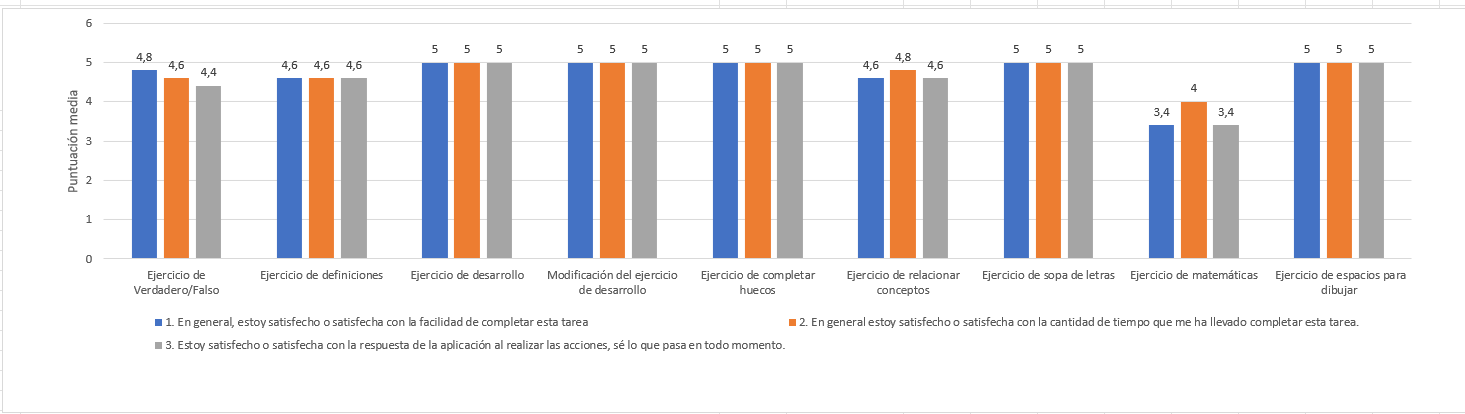
\includegraphics[width=\textwidth]{Evaluacion/GraficaResultadosExamen.png}
    \caption{Resultados de creación del examen.}
    \label{fig:resultadosExamen}
\end{figure}

En cuanto al apartado de la creación de una hoja de apuntes, los resultados obtenidos de cada tarea se muestran en las Tablas \ref{tab:pregunta1Apunte}, \ref{tab:pregunta2Apunte} y \ref{tab:pregunta3Apunte}. En el caso del resumen y el picotraductor se ha dado unas preguntas de respuesta abiertas para conocer su opinión sobre el resultado obtenido, esto lo podemos ver en la Tabla \ref{tab:OpinionResumen} y \ref{tab:OpinionPictotraductor}.

\begin{table}[H]
    \resizebox{\textwidth}{!}{%
        \begin{tabular}{c|cccccc|}
            \cline{2-7}
            \multicolumn{1}{l|}{}                                          & \multicolumn{6}{c|}{\textbf{1. En general, estoy satisfecho o satisfecha con la facilidad de completar esta tarea}}                                                                                                                                                                                          \\ \cline{2-7}
            \multicolumn{1}{l|}{}                                          & \multicolumn{1}{c|}{\textbf{Usuario 1}}                                                                             & \multicolumn{1}{c|}{\textbf{Usuario 2}} & \multicolumn{1}{c|}{\textbf{Usuario 3}} & \multicolumn{1}{c|}{\textbf{Usuario 4}} & \multicolumn{1}{c|}{\textbf{Usuario 5}} & \textbf{Media} \\ \hline
            \multicolumn{1}{|c|}{\textbf{Actividad 1: Resumen}}            & \multicolumn{1}{c|}{5}                                                                                              & \multicolumn{1}{c|}{5}                  & \multicolumn{1}{c|}{3}                  & \multicolumn{1}{c|}{5}                  & \multicolumn{1}{c|}{1}                  & \textbf{3,8}   \\ \hline
            \multicolumn{1}{|c|}{\textbf{Actividad 2: Leyenda de colores}} & \multicolumn{1}{c|}{3}                                                                                              & \multicolumn{1}{c|}{3}                  & \multicolumn{1}{c|}{1}                  & \multicolumn{1}{c|}{5}                  & \multicolumn{1}{c|}{1}                  & \textbf{2,6}   \\ \hline
            \multicolumn{1}{|c|}{\textbf{Actividad 3: Pictotraductor}}     & \multicolumn{1}{c|}{5}                                                                                              & \multicolumn{1}{c|}{5}                  & \multicolumn{1}{c|}{1}                  & \multicolumn{1}{c|}{5}                  & \multicolumn{1}{c|}{1}                  & \textbf{3,4}   \\ \hline
            \multicolumn{1}{|c|}{\textbf{Borrar una actividad}}            & \multicolumn{1}{c|}{5}                                                                                              & \multicolumn{1}{c|}{5}                  & \multicolumn{1}{c|}{3}                  & \multicolumn{1}{c|}{5}                  & \multicolumn{1}{c|}{1}                  & \textbf{3,8}   \\ \hline
            \multicolumn{1}{|c|}{\textbf{Actividad 4: Buscar pictogramas}} & \multicolumn{1}{c|}{5}                                                                                              & \multicolumn{1}{c|}{3}                  & \multicolumn{1}{c|}{4}                  & \multicolumn{1}{c|}{5}                  & \multicolumn{1}{c|}{1}                  & \textbf{3,6}   \\ \hline
        \end{tabular}%
    }
    \caption{Resultado de la pregunta de los apuntes: 1. En general, estoy satisfecho o satisfecha con la facilidad de completar esta tarea}
    \label{tab:pregunta1Apunte}
\end{table}

\begin{table}[H]
    \resizebox{\textwidth}{!}{%
        \begin{tabular}{c|cccccc|}
            \cline{2-7}
            \multicolumn{1}{l|}{}                                          & \multicolumn{6}{c|}{\textbf{\begin{tabular}[c]{@{}c@{}}2. En general estoy satisfecho o satisfecha con la cantidad de tiempo \\ que me ha llevado completar esta tarea.\end{tabular}}}                                                                                                                                                                                                               \\ \cline{2-7}
            \multicolumn{1}{l|}{}                                          & \multicolumn{1}{c|}{\textbf{Usuario 1}}                                                                                                                                                & \multicolumn{1}{l|}{\textbf{Usuario 2}} & \multicolumn{1}{l|}{\textbf{Usuario 3}} & \multicolumn{1}{l|}{\textbf{Usuario 4}} & \multicolumn{1}{l|}{\textbf{Usuario 5}} & \multicolumn{1}{l|}{\textbf{Media}} \\ \hline
            \multicolumn{1}{|c|}{\textbf{Actividad 1: Resumen}}            & \multicolumn{1}{c|}{0}                                                                                                                                                                 & \multicolumn{1}{c|}{5}                  & \multicolumn{1}{c|}{3}                  & \multicolumn{1}{c|}{5}                  & \multicolumn{1}{c|}{1}                  & \textbf{3,8}                        \\ \hline
            \multicolumn{1}{|c|}{\textbf{Actividad 2: Leyenda de colores}} & \multicolumn{1}{c|}{5}                                                                                                                                                                 & \multicolumn{1}{c|}{2}                  & \multicolumn{1}{c|}{1}                  & \multicolumn{1}{c|}{5}                  & \multicolumn{1}{c|}{1}                  & \textbf{2,8}                        \\ \hline
            \multicolumn{1}{|c|}{\textbf{Actividad 3: Pictotraductor}}     & \multicolumn{1}{c|}{5}                                                                                                                                                                 & \multicolumn{1}{c|}{5}                  & \multicolumn{1}{c|}{1}                  & \multicolumn{1}{c|}{5}                  & \multicolumn{1}{c|}{1}                  & \textbf{3,4}                        \\ \hline
            \multicolumn{1}{|c|}{\textbf{Borrar una actividad}}            & \multicolumn{1}{c|}{5}                                                                                                                                                                 & \multicolumn{1}{c|}{5}                  & \multicolumn{1}{c|}{3}                  & \multicolumn{1}{c|}{5}                  & \multicolumn{1}{c|}{1}                  & \textbf{3,8}                        \\ \hline
            \multicolumn{1}{|c|}{\textbf{Actividad 4: Buscar pictogramas}} & \multicolumn{1}{c|}{5}                                                                                                                                                                 & \multicolumn{1}{c|}{3}                  & \multicolumn{1}{c|}{4}                  & \multicolumn{1}{c|}{5}                  & \multicolumn{1}{c|}{1}                  & \textbf{3,6}                        \\ \hline
        \end{tabular}%
    }
    \caption{Resultado de la pregunta de los apuntes: 2. En general estoy satisfecho o satisfecha con la cantidad de tiempo que me ha llevado completar esta tarea.}
    \label{tab:pregunta2Apunte}
\end{table}

\begin{table}[H]
    \resizebox{\textwidth}{!}{%
        \begin{tabular}{c|cccccc|}
            \cline{2-7}
            \multicolumn{1}{l|}{}                                          & \multicolumn{6}{c|}{\textbf{\begin{tabular}[c]{@{}c@{}}3. Estoy satisfecho o satisfecha con la respuesta de la aplicación al \\ realizar las acciones, sé lo que pasa en todo momento.\end{tabular}}}                                                                                                                                                                                          \\ \cline{2-7}
            \multicolumn{1}{l|}{}                                          & \multicolumn{1}{c|}{\textbf{Usuario 1}}                                                                                                                                                               & \multicolumn{1}{c|}{\textbf{Usuario 2}} & \multicolumn{1}{c|}{\textbf{Usuario 3}} & \multicolumn{1}{c|}{\textbf{Usuario 4}} & \multicolumn{1}{c|}{\textbf{Usuario 5}} & \textbf{Media} \\ \hline
            \multicolumn{1}{|c|}{\textbf{Actividad 1: Resumen}}            & \multicolumn{1}{c|}{5}                                                                                                                                                                                & \multicolumn{1}{c|}{5}                  & \multicolumn{1}{c|}{3}                  & \multicolumn{1}{c|}{4}                  & \multicolumn{1}{c|}{1}                  & \textbf{3,6}   \\ \hline
            \multicolumn{1}{|c|}{\textbf{Actividad 2: Leyenda de colores}} & \multicolumn{1}{c|}{5}                                                                                                                                                                                & \multicolumn{1}{c|}{2}                  & \multicolumn{1}{c|}{1}                  & \multicolumn{1}{c|}{5}                  & \multicolumn{1}{c|}{1}                  & \textbf{2,8}   \\ \hline
            \multicolumn{1}{|c|}{\textbf{Actividad 3: Pictotraductor}}     & \multicolumn{1}{c|}{5}                                                                                                                                                                                & \multicolumn{1}{c|}{2}                  & \multicolumn{1}{c|}{1}                  & \multicolumn{1}{c|}{5}                  & \multicolumn{1}{c|}{1}                  & \textbf{2,8}   \\ \hline
            \multicolumn{1}{|c|}{\textbf{Borrar una actividad}}            & \multicolumn{1}{c|}{5}                                                                                                                                                                                & \multicolumn{1}{c|}{4}                  & \multicolumn{1}{c|}{3}                  & \multicolumn{1}{c|}{5}                  & \multicolumn{1}{c|}{1}                  & \textbf{3,6}   \\ \hline
            \multicolumn{1}{|c|}{\textbf{Actividad 4: Buscar pictogramas}} & \multicolumn{1}{c|}{5}                                                                                                                                                                                & \multicolumn{1}{c|}{4}                  & \multicolumn{1}{c|}{4}                  & \multicolumn{1}{c|}{5}                  & \multicolumn{1}{c|}{1}                  & \textbf{3,8}   \\ \hline
        \end{tabular}%
    }
    \caption{Resultado de la pregunta de los apuntes: 3. Estoy satisfecho o satisfecha con la respuesta de la aplicación al realizar las acciones, sé lo que pasa en todo momento.}
    \label{tab:pregunta3Apunte}
\end{table}

% Opiniones

\begin{table}[H]
    \resizebox{\textwidth}{!}{%
        \begin{tabular}{|cc|}
            \hline
            \multicolumn{2}{|c|}{\textbf{Actividad 1: Resumen}}                                                                                                                              \\ \hline
            \multicolumn{1}{|c|}{\textbf{¿ El resumen resultante te parece correcto?}} & \textbf{¿Qué cuestiones crees que son mejorables en el resumen o que no son correctas?}             \\ \hline
            \multicolumn{1}{|c|}{No}                                                   & Está muy bien. Lo ha resumido mejor de lo que pensaba                                               \\ \hline
            \multicolumn{1}{|c|}{Sí}                                                   & Es mejorable la redacción en cuanto a signos de puntuación y conectores para dar cohesión al texto. \\ \hline
            \multicolumn{1}{|c|}{Sí}                                                   & No he visto dónde especificar que quería 100 palabras.                                              \\ \hline
            \multicolumn{1}{|c|}{Sí}                                                   & Se podrían seleccionar palabras que deseemos que salgan obligatoriamente en el resumen.             \\ \hline
            \multicolumn{1}{|c|}{No}                                                   & El programa no me ha hecho el resumen. Se quedaba bloqueado.                                        \\ \hline
        \end{tabular}%
    }
    \caption{Evaluación funcionalidad resumen}
    \label{tab:OpinionResumen}
\end{table}

\begin{table}[H]
    \resizebox{\textwidth}{!}{%
        \begin{tabular}{|c|}
            \hline
            \textbf{Actividad 3: Pictotraductor}                                                                                                                                                                                                                                                                                                                                                                                                                                            \\ \hline
            \textbf{¿Qué cuestiones crees que son mejorables en la traducción o que no son correctas?}                                                                                                                                                                                                                                                                                                                                                                                      \\ \hline
            no sulen emplearse artículos en las traducciones de pictogramas, pero está bien                                                                                                                                                                                                                                                                                                                                                                                                 \\ \hline
            \begin{tabular}[c]{@{}c@{}}Los artículos son complejos de entender mediante dibujos. \\ En ocasiones se podrían omitir, puesto que si leemos \\ "En boca alimentos mezclan con saliva" \\ la frase seguiría teniendo sentido. O los destinatarios de estos \\ ejercicios tienen muy claro que dichos pictogramas corresponden \\ a artículos, o podrían confundirse con otras palabras. Es fantástica la opción \\ de omitir o no poner visibles algunos de ellos.\end{tabular} \\ \hline
            \begin{tabular}[c]{@{}c@{}}No aparecen (o yo no encuentro) todos los pictogramas \\ que ponéis en el resultado que debe salir. \\ Normalmente, no se deben "traducir" \\ todas las palabras, sólo sustantivos y/o las\\  más significativas.\end{tabular}                                                                                                                                                                                                                       \\ \hline
            Son correctas.                                                                                                                                                                                                                                                                                                                                                                                                                                                                  \\ \hline
            No me ha buscado nada                                                                                                                                                                                                                                                                                                                                                                                                                                                           \\ \hline
        \end{tabular}%
    }
    \caption{Evaluación funcionalidad pictotraductor}
    \label{tab:OpinionPictotraductor}
\end{table}

\begin{table}[H]
    \resizebox{\textwidth}{!}{%
        \begin{tabular}{c|cccccc|}
            \cline{2-7}
            \multicolumn{1}{l|}{}                                          & \multicolumn{6}{c|}{\textbf{\begin{tabular}[c]{@{}c@{}}3. Estoy satisfecho o satisfecha con la respuesta de la aplicación al \\ realizar las acciones, sé lo que pasa en todo momento.\end{tabular}}}                                                                                                                                                                                                               \\ \cline{2-7}
            \multicolumn{1}{l|}{}                                          & \multicolumn{1}{c|}{\textbf{Usuario 1}}                                                                                                                                                               & \multicolumn{1}{l|}{\textbf{Usuario 2}} & \multicolumn{1}{l|}{\textbf{Usuario 3}} & \multicolumn{1}{l|}{\textbf{Usuario 4}} & \multicolumn{1}{l|}{\textbf{Usuario 5}} & \multicolumn{1}{l|}{\textbf{Media}} \\ \hline
            \multicolumn{1}{|c|}{\textbf{Actividad 1: Resumen}}            & \multicolumn{1}{c|}{5}                                                                                                                                                                                & \multicolumn{1}{c|}{5}                  & \multicolumn{1}{c|}{3}                  & \multicolumn{1}{c|}{4}                  & \multicolumn{1}{c|}{1}                  & \textbf{3,6}                        \\ \hline
            \multicolumn{1}{|c|}{\textbf{Actividad 2: Leyenda de colores}} & \multicolumn{1}{c|}{5}                                                                                                                                                                                & \multicolumn{1}{c|}{2}                  & \multicolumn{1}{c|}{1}                  & \multicolumn{1}{c|}{5}                  & \multicolumn{1}{c|}{1}                  & \textbf{2,8}                        \\ \hline
            \multicolumn{1}{|c|}{\textbf{Actividad 3: Pictotraductor}}     & \multicolumn{1}{c|}{5}                                                                                                                                                                                & \multicolumn{1}{c|}{2}                  & \multicolumn{1}{c|}{1}                  & \multicolumn{1}{c|}{5}                  & \multicolumn{1}{c|}{1}                  & \textbf{2,8}                        \\ \hline
            \multicolumn{1}{|c|}{\textbf{Borrar una actividad}}            & \multicolumn{1}{c|}{5}                                                                                                                                                                                & \multicolumn{1}{c|}{4}                  & \multicolumn{1}{c|}{3}                  & \multicolumn{1}{c|}{5}                  & \multicolumn{1}{c|}{1}                  & \textbf{3,6}                        \\ \hline
            \multicolumn{1}{|c|}{\textbf{Actividad 4: Buscar pictogramas}} & \multicolumn{1}{c|}{5}                                                                                                                                                                                & \multicolumn{1}{c|}{4}                  & \multicolumn{1}{c|}{4}                  & \multicolumn{1}{c|}{5}                  & \multicolumn{1}{c|}{1}                  & \textbf{3,8}                        \\ \hline
        \end{tabular}%
    }
    \caption{Resultado de la pregunta de los apuntes: 3. Estoy satisfecho o satisfecha con la respuesta de la aplicación al realizar las acciones, sé lo que pasa en todo momento.}
    \label{tab:pregunta3Apunte}
\end{table}

\begin{table}[H]
    \resizebox{\textwidth}{!}{
        \begin{tabular}{l|c|c|c|}
            \cline{2-4}
                                                                            & \textbf{\begin{tabular}[c]{@{}l@{}}1.   En general, estoy satisfecho o \\ satisfecha con la facilidad de \\ completar esta   tarea.\end{tabular}} & \textbf{\begin{tabular}[c]{@{}l@{}}2.   En general estoy satisfecho o \\ satisfecha con la cantidad de tiempo \\ que me ha llevado completar \\ esta tarea.\end{tabular}} & \textbf{\begin{tabular}[c]{@{}l@{}}3.   Estoy satisfecho o satisfecha con \\ la respuesta de la aplicación al \\ realizar las acciones, sé lo que \\ pasa en todo momento.\end{tabular}} \\ \hline
            \multicolumn{1}{|l|}{\textbf{Actividad 1: Resumen}}             & 3,8                                                                                                                                               & 3,8                                                                                                                                                                       & 3,6                                                                                                                                                                                      \\ \hline
            \multicolumn{1}{|l|}{\textbf{Actividad  2: Leyenda de colores}} & 2,6                                                                                                                                               & 2,8                                                                                                                                                                       & 2,8                                                                                                                                                                                      \\ \hline
            \multicolumn{1}{|l|}{\textbf{Actividad 3: Pictotraductor}}      & 3,4                                                                                                                                               & 3,4                                                                                                                                                                       & 3,2                                                                                                                                                                                      \\ \hline
            \multicolumn{1}{|l|}{\textbf{Borrar una actividad}}             & 3,8                                                                                                                                               & 3,8                                                                                                                                                                       & 3,6                                                                                                                                                                                      \\ \hline
            \multicolumn{1}{|l|}{\textbf{Actividad 4: Buscar pictogramas}}  & 3,6                                                                                                                                               & 3,6                                                                                                                                                                       & 3,6                                                                                                                                                                                      \\ \hline
        \end{tabular}
    }
    \caption{Resultados de la creación de la hoja de apuntes}
    \label{tab:resultadosApuntes}
\end{table}

\begin{figure}[ht!]
    \centering
    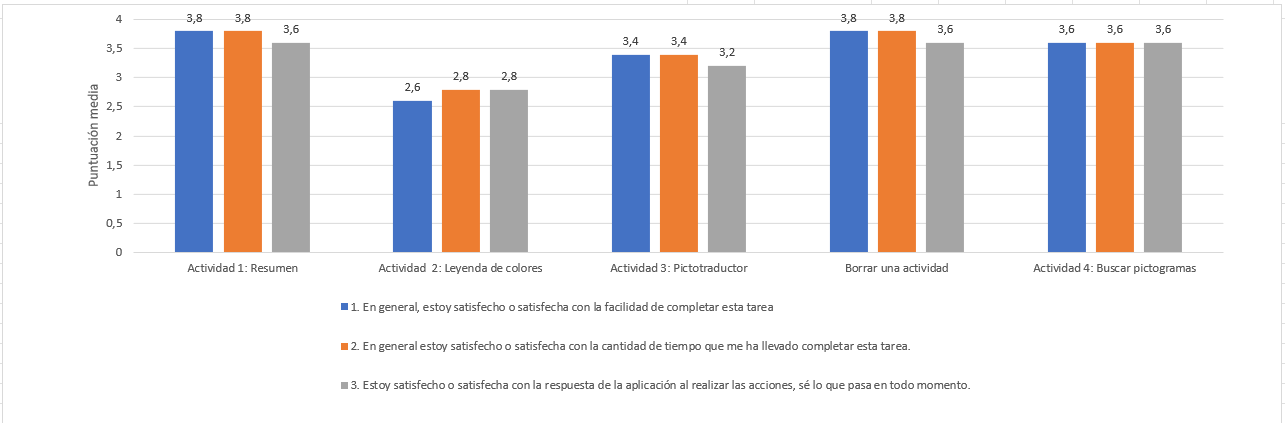
\includegraphics[width=\textwidth]{Evaluacion/GraficaResultadosApuntes.png}
    \caption{Resultados de creación de la hoja de apuntes.}
    \label{fig:resultadosApuntes}
\end{figure}

En cuanto a las preguntas del cuestionario SUS, la puntuación final obtenida fue de 78,5. Esta puntuación indica que el sistema todavía requiere mejoras. Los detalles del cálculo se encuentran en la tabla \ref{tab:puntuacionSUS}.

\begin{table}[H]
    \resizebox{\textwidth}{!}{%
        \begin{tabular}{c|c|c|c|c|c|c|}
            \cline{2-7}
            \multicolumn{1}{l|}{}                                                                                                                                                     & \textbf{Usuario 1} & \textbf{Usuario 2} & \textbf{Usuario 3} & \textbf{Usuario 4} & \textbf{Usuario 5} & \textbf{Media:} \\ \hline
            \multicolumn{1}{|c|}{\textbf{Creo que usaría esta aplicación frecuentemente.}}                                                                                            & 5                  & 4                  & 4                  & 5                  & 2                  & \textbf{4}      \\ \hline
            \multicolumn{1}{|c|}{\textbf{Encontré la aplicación innecesariamente compleja}}                                                                                           & 1                  & 2                  & 2                  & 1                  & 3                  & \textbf{1,8}    \\ \hline
            \multicolumn{1}{|c|}{\textbf{Creo que la aplicación es fácil de usar}}                                                                                                    & 4                  & 4                  & 4                  & 5                  & 3                  & \textbf{4}      \\ \hline
            \multicolumn{1}{|c|}{\textbf{\begin{tabular}[c]{@{}c@{}}Creo que necesitaría la ayuda de una persona \\ con conocimientos técnicos para usar la aplicación\end{tabular}}} & 5                  & 1                  & 1                  & 1                  & 2                  & \textbf{2}      \\ \hline
            \multicolumn{1}{|c|}{\textbf{Las funciones de la aplicación están bien integradas}}                                                                                       & 5                  & 4                  & 4                  & 5                  & 2                  & \textbf{4}      \\ \hline
            \multicolumn{1}{|c|}{\textbf{Creo que la aplicación es muy confusa}}                                                                                                      & 2                  & 2                  & 2                  & 1                  & 3                  & \textbf{2}      \\ \hline
            \multicolumn{1}{|c|}{\textbf{\begin{tabular}[c]{@{}c@{}}Creo que la mayoría de la gente aprendería a usar \\ la aplicación muy rápidamente\end{tabular}}}                 & 5                  & 4                  & 5                  & 4                  & 4                  & \textbf{4,4}    \\ \hline
            \multicolumn{1}{|c|}{\textbf{Encuentro la aplicación muy complicada de utilizar}}                                                                                         & 1                  & 5                  & 1                  & 1                  & 2                  & \textbf{2}      \\ \hline
            \multicolumn{1}{|c|}{\textbf{Me siento confiado o confiada al utilizar la aplicación}}                                                                                    & 5                  & 5                  & 5                  & 5                  & 3                  & \textbf{4,6}    \\ \hline
            \multicolumn{1}{|c|}{\textbf{\begin{tabular}[c]{@{}c@{}}Necesito aprender muchas cosas antes de \\ poder utilizar la aplicación\end{tabular}}}                            & 1                  & 1                  & 1                  & 4                  & 2                  & \textbf{1,8}    \\ \hline
            \multicolumn{1}{|c|}{\textbf{Resultado}}                                                                                                                                  & \textbf{85}        & \textbf{75}        & \textbf{87,5}      & \textbf{90}        & \textbf{55}        & \textbf{78,5}   \\ \hline
        \end{tabular}%
    }
    \caption{Resultado del cuestionario SUS}
    \label{tab:puntuacionSUS}
\end{table}

Finalmente los usuarios han compartido sus opiniones sobre la aplicación. En general, el ``Usuario 1'' considera que la aplicación es muy buena y útil. Lo que más le ha gustado son las opciones novedosas e intuitivas, como la capacidad de hacer resúmenes y buscar pictogramas en un texto. Sin embargo, le ha decepcionado no poder editar el texto como en un procesador de texto y la falta de una opción de deshacer o retroceder. Por otro lado, el ``Usuario 2'' opina que la herramienta es muy útil para el profesorado en general. Destaca especialmente las opciones de ejercicios, como la sopa de letras, completar huecos en blanco y relacionar conceptos. Sin embargo, menciona que ha tenido dificultades al aplicar colores a la leyenda y echa de menos una herramienta de deshacer En cuanto al ``Usuario 3'' , encuentra la aplicación bastante completa, pero echa en falta una opción de ayuda para entender cada ejercicio. Lo que más le ha gustado es la facilidad de redacción y realización de los ejercicios una vez que se entienden. No obstante, menciona que ha perdido tiempo al haber redactado su propio examen y luego encontrarse con ejercicios tipo al pasar de página. El ``Usuario 4'' opina que la aplicación es muy útil para la elaboración de actividades. Destaca la variedad de opciones que ofrece. Sin embargo, considera confusa la parte de Matemáticas. Por último, el ``Usuario 5'' encuentra la aplicación interesante, pero menciona limitaciones y problemas de funcionamiento. Lo que más le ha gustado es la facilidad para hacer crucigramas. Sin embargo, ha experimentado problemas al traducir a pictogramas y no ha podido resumir un texto. Además, le gustaría poder mover los ejercicios y tener un documento menos estructurado.

\section{Conclusiones}\label{sec:conclusionesEvaluacion}
Tras evaluar la aplicación web AdaptaMaterialEscolar 2.0, hemos determinado que, aunque existen áreas de mejora, el sistema presenta una usabilidad satisfactoria, con una puntuación de 78.5 sobre 100 (Tabla \ref{tab:puntuacionSUS}). Esta puntuación indica que el sistema se considera fácil de usar y los usuarios están satisfechos.

En cuanto a las funcionalidades para generar ejercicios, la evaluación refleja que la facilidad para completar las tareas es alta, ya que todas las puntuaciones promedio para la pregunta ``facilidad de completar esta tarea'' están por encima de 4 (Figura \ref{fig:resultadosExamen}). La cantidad de tiempo requerido para completar las tareas también es en su mayoría satisfactoria, ya que todas las puntuaciones promedio para la pregunta ``cantidad de tiempo que me ha llevado completar esta tarea'' son iguales o superiores a 4 (Figura \ref{fig:resultadosExamen}). Las puntuaciones promedio para la pregunta ``respuesta de la aplicación al realizar las acciones, sé lo que pasa en todo momento'' son de 5, lo cual indica que los usuarios están muy satisfechos con la respuesta de la aplicación y su capacidad de comprender lo que ocurre (Figura \ref{fig:resultadosExamen}). Además, observamos que el ejercicio de desarrollo, la modificación del ejercicio de desarrollo, el ejercicio de completar huecos, el ejercicio de sopa de letras y el ejercicio para espacio para dibujar obtienen la puntuación más alta, mientras que el ejercicio de completar huecos cuenta con la puntuación más baja.

Por otro lado, las funcionalidades para crear apuntes muestran un grado de satisfacción moderado en cuanto a la facilidad, la respuesta de la aplicación y el tiempo requerido para completar las tareas. Sin embargo, existe un amplio margen de mejora, dado que todas las actividades obtienen una puntuación promedio superior a 3 en una escala del 1 al 5 (Figura \ref{fig:resultadosApuntes}). Esto indica que los usuarios se sienten satisfechos con las funcionalidades de creación de apuntes, pero consideran que aún se pueden realizar mejoras.

Es importante destacar que los usuarios se mostraron más cómodos con las funcionalidades relacionadas con la generación de ejercicios de examen (Figura \ref{fig:graficaComparativaEjerciciosApuntes}) que con las de adaptación de texto.

\begin{figure}[ht!]
    \centering
    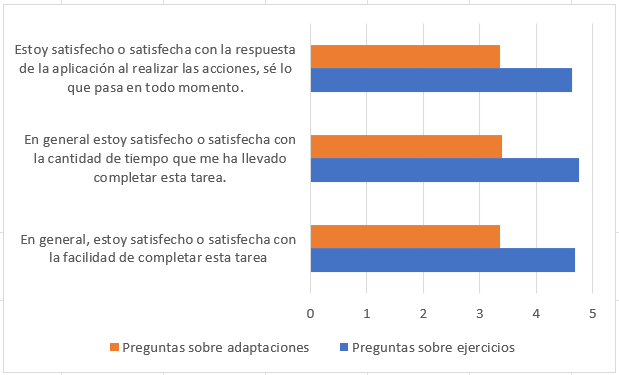
\includegraphics[width=0.75\textwidth]{Evaluacion/GraficaComparativaEjerciciosApuntes.png}
    \caption{Gráfica comparativa entre ejercicios y apuntes.}
    \label{fig:graficaComparativaEjerciciosApuntes}
\end{figure}

Por último, se han analizado las respuestas a las preguntas sobre la opinión de los usuarios. En líneas generales, los usuarios consideran que AdaptaMaterialEscolar 2.0 es una herramienta muy interesante y útil, pero mejoras. Las ideas de mejora y nuevos requisitos obtenidos como resultado de la evaluación son los siguientes:

\begin{itemize}
    \item Posibilidad de reorganizar los ejercicios. Los evaluadores echaron de menos poder cambiar el orden de los ejercicios.
    \item Permitir deshacer y rehacer cualquier acción para de este modo hacer sentir al usuario en control de la aplicación y que pueda explorarla sin miedo a equivocarse. Esta nueva funcionalidad además permitiría al usuario recuperarse fácilmente de los errores.
    \item Añadir ayuda en todas las funcionalidades de la aplicación.
    \item Permitir la selección de palabras específicas para que aparezcan obligatoriamente en el resumen.
    \item Mejorar la redacción en cuanto a signos de puntuación y conectores para dar cohesión al texto.
    \item Al traducir un texto a pictogramas se debería omitir los artículos ya que son complejos de entender mediante dibujos.
    \item Mejorar la edición de los ejercicios en el documento de trabajo.
    \item Posibilidad de generar ejercicios no numerados.
    \item Mejorar las funcionales de edición de texto avanzado.
    \item Permitir asignar colores automáticamente al texto según las categorías seleccionadas en la leyenda de colores.
    \item Mejorar la funcionalidad de ejercicios de matemáticas ya que los evaluadores la consideran confusa.
\end{itemize}